\section{Υπολογισμός παραγώγων ευαισθησίας με πεπερασμένες διαφορές}

Οι πεπερασμένες διαφορές αποτελούν την πιο απλή αλλά και υπολογιστική απαιτητική μέθοδο υπολογισμού των παραγώγων ευαισθησίας. Για τον υπολογισμό των παραγώγων, χρησιμοποιούμε κεντρικές πεπερασμένες διαφορες. Μεταβάλλουμε την τιμή της υπο μελέτη μεταβλητής κατά μια μικρή ποσότητα $\epsilon$ και υπολογίζουμε την μεταβολή που προκαλεί στην αντικειμενική συνάρτηση. Φύσικα, όπως και προηγουμένως, ο καθορισμός ενος ικανοποιητικού βήματος $\epsilon$ απαιτεί μια ανάλυση ανεξαρτησίας των αποτελεσμάτων απο την ποσότητα αυτή.



Η διαδικασία υπολογισμού των παραγώγων παρατίθεται στο σχήμα \ref{fig:fdcode} μέσω ενός τμήματος του κώδικα.
%\subfile{3-1_FD_Code}

\begin{figure}[h!]
\centering
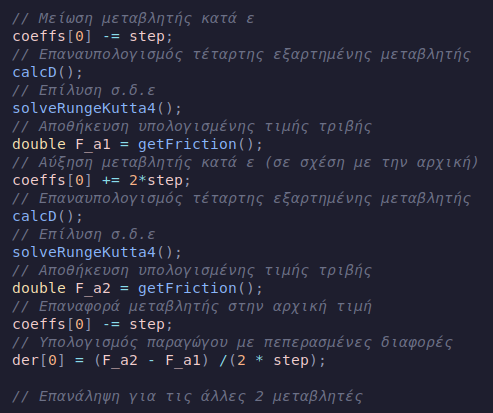
\includegraphics[height=.5\textwidth]{figures/FD_code.png}
\caption{Τυπική μεθοδολογία υπολογιμού παραγώγων με πεπερασμένες διαφορές}
\label{fig:fdcode}
\end{figure}

Η εξάρτηση μίας εκ των τριών παραγώγων ευαισθησίας απο το μέγεθος του βήματος φαίνεται στο σχήμα \ref{fig:fdstep}. Η συμπεριφορά των άλλων δυο παραγώγων είναι ανάλογη αυτής του σχήματος \ref{fig:fdstep}.


\begin{figure}[h!]
\centering
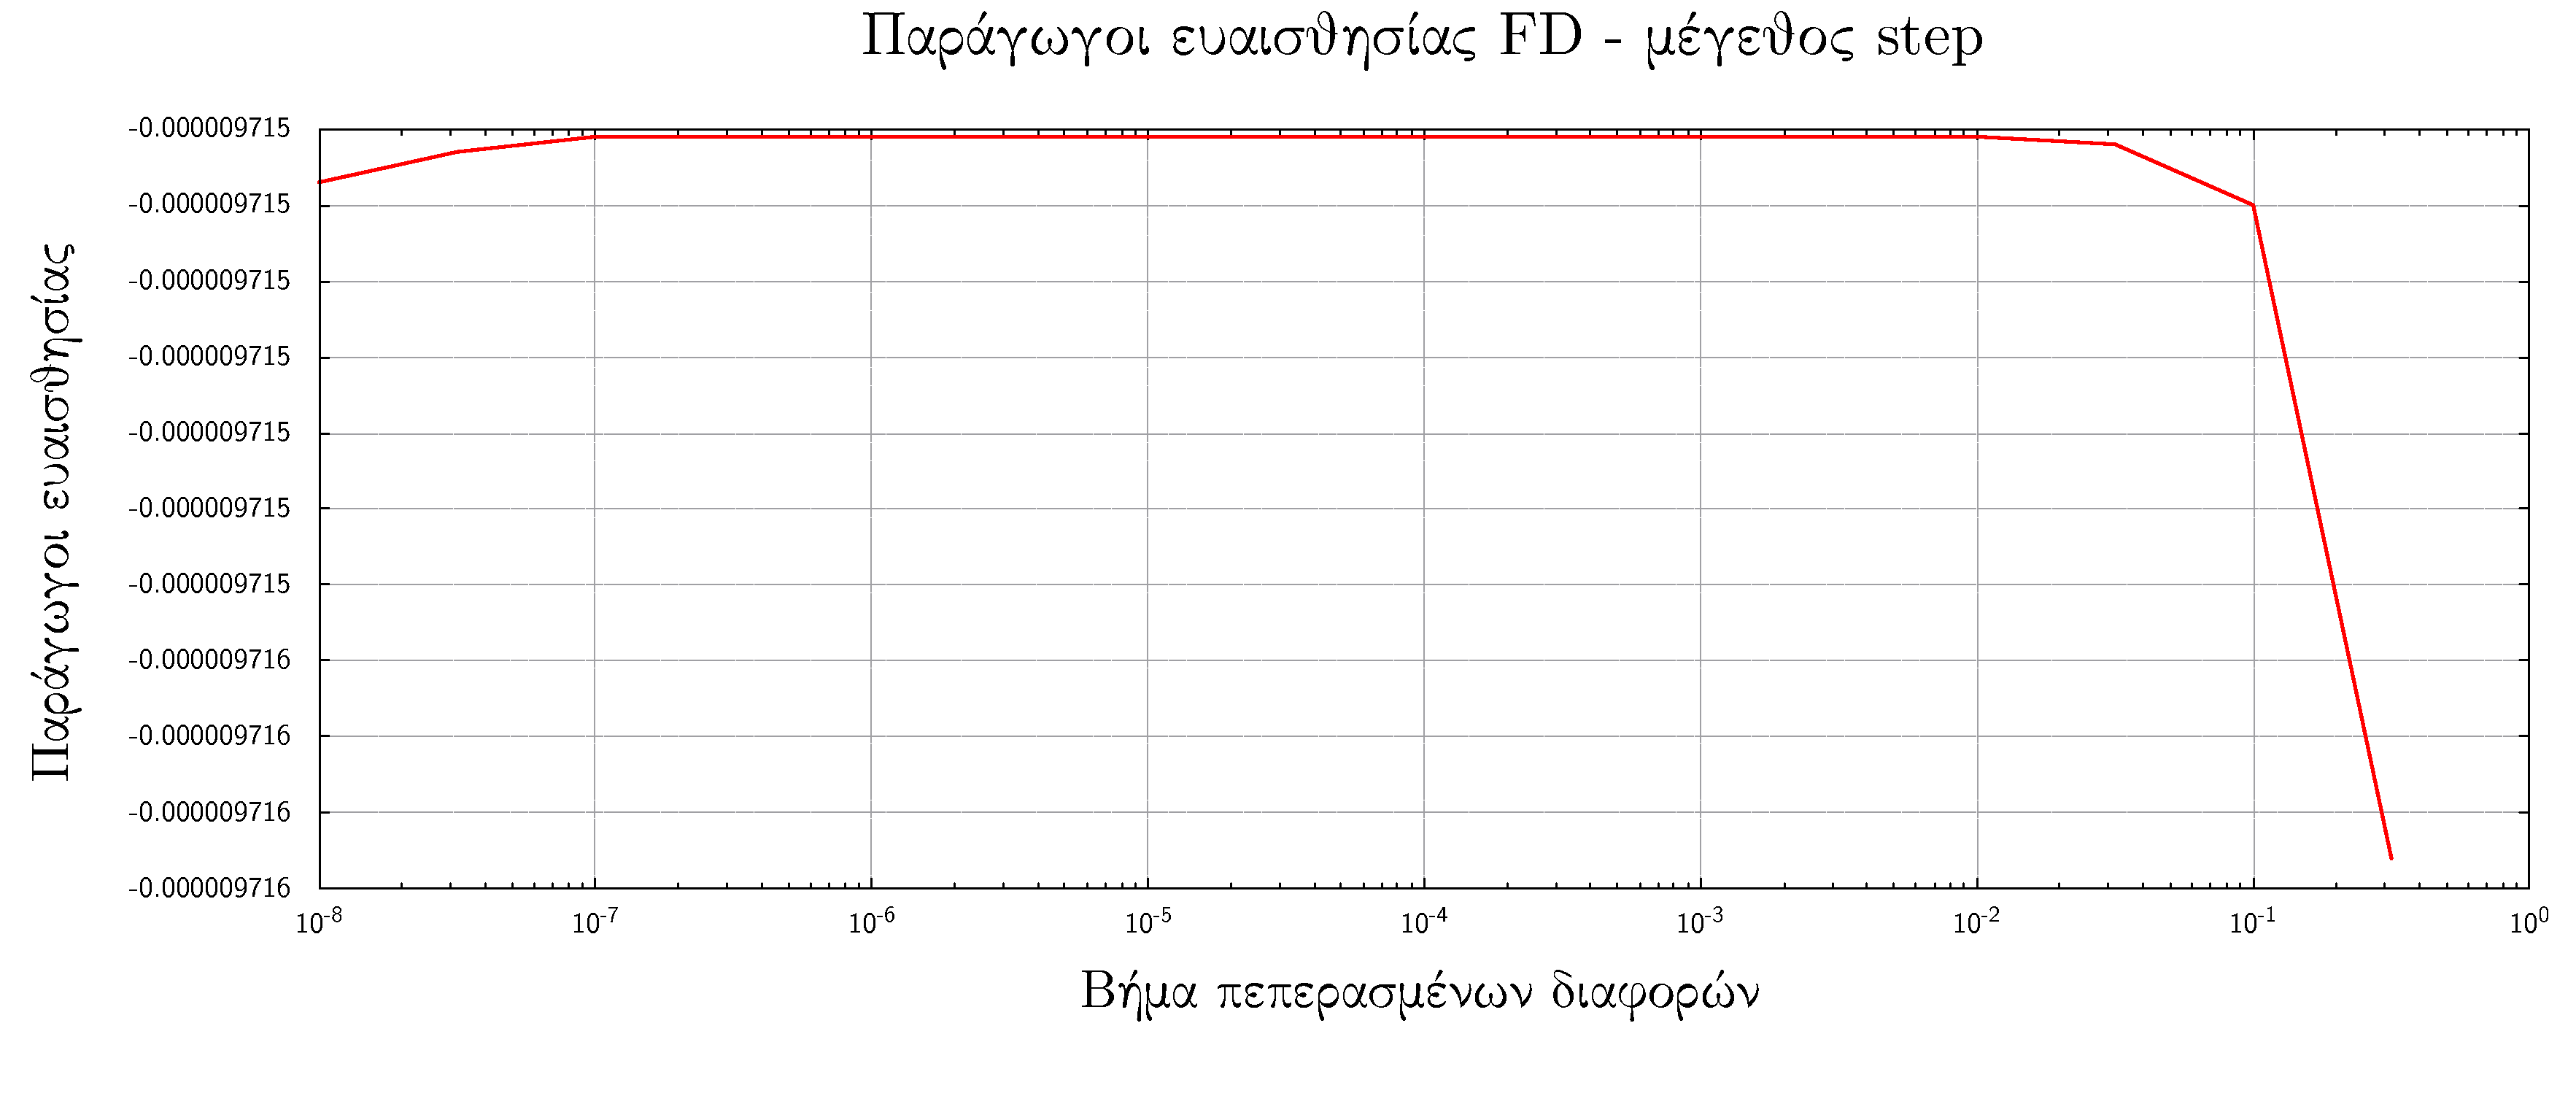
\includegraphics[width=.8\textwidth]{figures/fd_step.pdf}
\caption{Εξάρτηση της παραγώγου απο το βήμα των πεπερασμένων διαφορών}
\label{fig:fdstep}
\end{figure}

Παρατηρούμε πως ξεκινώντας απο βήμα της τάξης των $10^{-1}$ και μειώνωντας το βήμα, η τιμή της παραγώγου σταθεροποιείται, διατηρώντας σχεδόν σταθερή τιμή για βήμα μικρότερο του $10^{-2}$. Ωστόσο παρατηρούμε πως για πολύ μικρό βήμα, της τάξης του $10^{-8}$, εμφανίζονται σφάλματα αποκοπής λόγω της αναπαράστασης των αριθμών και μεταβάλλονται τα αποτελέσματα. Έτσι, για βήμα της τάξης του $10^{-3}$ μπορούμε να αποφανθούμε πως έχουμε αρκετά αξιόπιστο υπολογισμό των παραγώγων.


